\documentclass[tikz,border=6pt]{standalone}
\usetikzlibrary{arrows.meta}
\begin{document}
% New construction for UDL Problem 3.16, following Figure 3.11's visual convention.
% Two inputs, four ReLU hidden units, three affine outputs; every adjacent pair
% of layers is fully connected. Biases appear in the equations, not as nodes.
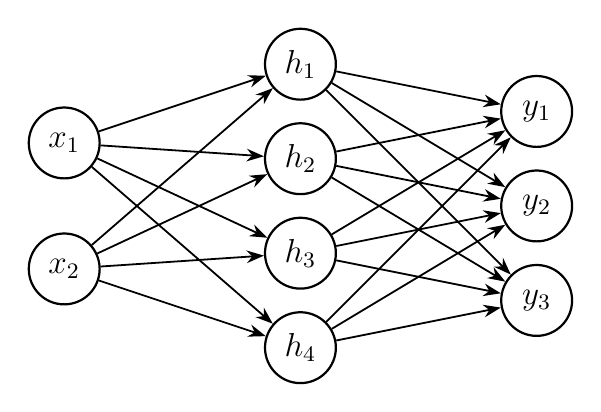
\begin{tikzpicture}[
  unit/.style={circle,draw=black,line width=.8pt,minimum size=9mm,inner sep=0pt,fill=white,font=\large},
  connection/.style={-{Stealth[length=2.2mm,width=1.6mm]},line width=.65pt}
]
\node[unit] (x1) at (0,.8) {$x_1$};
\node[unit] (x2) at (0,-.8) {$x_2$};
\foreach \j/\y in {1/1.8,2/.6,3/-.6,4/-1.8}
  \node[unit] (h\j) at (3,\y) {$h_\j$};
\foreach \k/\y in {1/1.2,2/0,3/-1.2}
  \node[unit] (y\k) at (6,\y) {$y_\k$};
\foreach \i in {1,2}
  \foreach \j in {1,2,3,4}
    \draw[connection] (x\i) -- (h\j);
\foreach \j in {1,2,3,4}
  \foreach \k in {1,2,3}
    \draw[connection] (h\j) -- (y\k);
\end{tikzpicture}
\end{document}
